\documentclass[tikz]{standalone}
\usepackage{tikz}
\usetikzlibrary{shapes,calc,arrows,through,intersections,angles}
\usepackage{xcolor}
\usepackage{pgfplots}
\pgfplotsset{compat=1.8}
\usepackage{nicefrac}

\begin{document}

%----Proper document------------------------------------------------------------

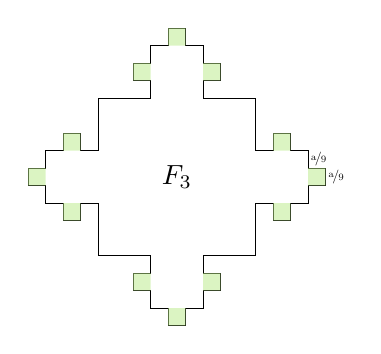
\begin{tikzpicture}[scale=2/9]
	\definecolor{limegreen}{RGB}{184,233,134}

	\draw (0,0) -- (3,0) -- (3,-1) -- (2,-1) -- (2,-2) -- (3,-2) -- (3,-3) -- (4,-3) -- (4,-4) -- (5,-4) -- (5,-3) -- (6,-3) -- (6,-2) -- (7,-2) -- (7,-1) -- (6,-1) -- (6,0) -- (9,0);
	\fill [fill=limegreen, opacity=0.5] (2,-2) -- (3,-2) -- (3,-1) -- (2,-1) -- (2,-2);
	\fill [fill=limegreen, opacity=0.5] (4,-4) -- (5,-4) -- (5,-3) -- (4,-3) -- (4,-4);
	\fill [fill=limegreen, opacity=0.5] (6,-2) -- (7,-2) -- (7,-1) -- (6,-1) -- (6,-2);

    \begin{scope}[shift={(9,0)},rotate=90]
        \draw (0,0) -- (3,0) -- (3,-1) -- (2,-1) -- (2,-2) -- (3,-2) -- (3,-3) -- (4,-3) -- (4,-4) -- (5,-4) -- (5,-3) -- (6,-3) -- (6,-2) -- (7,-2) -- (7,-1) -- (6,-1) -- (6,0) -- (9,0);
		\fill [fill=limegreen, opacity=0.5] (2,-2) -- (3,-2) -- (3,-1) -- (2,-1) -- (2,-2);
		\fill [fill=limegreen, opacity=0.5] (4,-4) -- (5,-4) -- (5,-3) -- (4,-3) -- (4,-4);
		\fill [fill=limegreen, opacity=0.5] (6,-2) -- (7,-2) -- (7,-1) -- (6,-1) -- (6,-2);
    \end{scope}

    \begin{scope}[shift={(9,9)},rotate=180]
        \draw (0,0) -- (3,0) -- (3,-1) -- (2,-1) -- (2,-2) -- (3,-2) -- (3,-3) -- (4,-3) -- (4,-4) -- (5,-4) -- (5,-3) -- (6,-3) -- (6,-2) -- (7,-2) -- (7,-1) -- (6,-1) -- (6,0) -- (9,0);
		\fill [fill=limegreen, opacity=0.5] (2,-2) -- (3,-2) -- (3,-1) -- (2,-1) -- (2,-2);
		\fill [fill=limegreen, opacity=0.5] (4,-4) -- (5,-4) -- (5,-3) -- (4,-3) -- (4,-4);
		\fill [fill=limegreen, opacity=0.5] (6,-2) -- (7,-2) -- (7,-1) -- (6,-1) -- (6,-2);
    \end{scope}

    \begin{scope}[shift={(0,9)},rotate=270]
        \draw (0,0) -- (3,0) -- (3,-1) -- (2,-1) -- (2,-2) -- (3,-2) -- (3,-3) -- (4,-3) -- (4,-4) -- (5,-4) -- (5,-3) -- (6,-3) -- (6,-2) -- (7,-2) -- (7,-1) -- (6,-1) -- (6,0) -- (9,0);
		\fill [fill=limegreen, opacity=0.5] (2,-2) -- (3,-2) -- (3,-1) -- (2,-1) -- (2,-2);
		\fill [fill=limegreen, opacity=0.5] (4,-4) -- (5,-4) -- (5,-3) -- (4,-3) -- (4,-4);
		\fill [fill=limegreen, opacity=0.5] (6,-2) -- (7,-2) -- (7,-1) -- (6,-1) -- (6,-2);
    \end{scope}

    \node at (13.6,4.5) {$\scalebox{0.5}{\nicefrac{a}{9}}$};
    \node at (12.6,5.5) {$\scalebox{0.5}{\nicefrac{a}{9}}$};
	\node at (4.5,4.5) {$F_3$};
\end{tikzpicture}

%-------------------------------------------------------------------------------

\end{document}
